% vqa.tex

% definition
With the goal of optimizing learning computations using quantum computers in
mind, we need an abstract idea of how to implement this connection. A
\emph{Variational Quantum Algorithm} (VQA) is any such system based on a
proposed architecture for a classically controlled quantum computer
\cite{bharti2021noisy}. \autoref{fig:vqaarch} presents the proposed
architecture. The following subsection presents an expanded view of the
computation.

% hybrid diagram
\begin{figure}
    \centering
    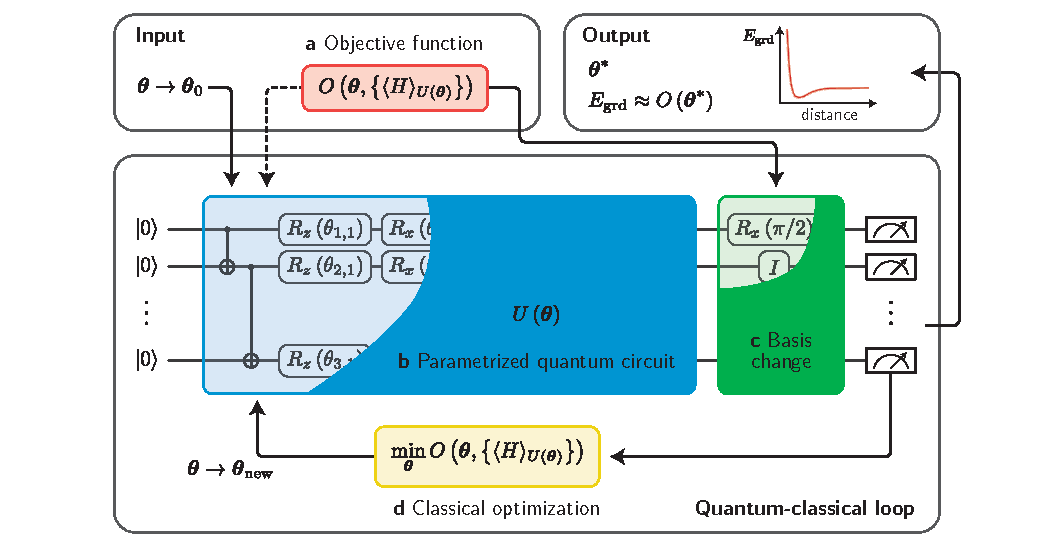
\includegraphics[width=\textwidth]{figures/vqaarch.pdf}
    \caption{Diagrammatic representation of a Variational Quantum Algorithm
    (VQA) \cite[see][chapter 2]{bharti2021noisy}.}
    \label{fig:vqaarch}
\end{figure}


\subsection{Building Blocks}

A VQA computation has 4 major components, as shown in \autoref{fig:vqaarch}:

\begin{itemize}
    \item objective function --- the encoding of the problem at hand as an
            optimization,
    \item parametrized quantum circuit (PQC) --- circuit encoding a unitary
            operator parametrized by classically controlled parameters
            \(\vec{\theta}\),
    \item measurement scheme --- the system performing basis changes and
            transferring outputs to the control system, and
    \item classical optimizer --- a classical objective minimizer which controls
            the PQC.
\end{itemize}

These components form a modular computation model where each of the components
can be swapped and improved individually to relieve bottnecks and adapt to the
problem at hand, to control the expressiveness of the system or avoid
treacherous optimization landscapes \cite{larocca2021theory}.

\subsubsection{Objective Function}

The \emph{objective} or \emph{loss function} \cite{larocca2021theory} forms the
target of the optimization problem at hand. This can be any function that can be
encoded in an operational form, i.e., written as or decomposed into quantum
operators. In most cases, this can be expected to be something akin to the
Hamiltonian of a system \cite{bharti2021noisy}, thus making the minimal, ground
state, energy the optimization target. This may also be called the
\emph{parametrized cost} of the computation. Subject to the optimization
constraints, the target of the system is then to find the optimal parameter
input
\begin{gather*}
    % stupid \min isn't working with subcript for some reason
    \parameters_* = \text{arg min}_\parameters\;{\loss(\parameters, p_0(\parameters))}~,
\end{gather*}

where \(p_0(\parameters)\) represents the parametrised probability to measure
the output in the state \(\ket*{0}\).

% pqc
\subsubsection{Parametrised Quantum Circuits (PQCs)}
The module central to the computation is the parametrised quantum circuit given
by \(\pqc(\parameters)\). It is the component of the circuit which performs the
actual `computation' and outputs the state that best meets the objective. It
does so by acting on the input state a series of unitary transformations
parametrised by controllable inputs. We assume the circuit to have an
\(L\)-layered structure as

\begin{gather}
    \pqc(\parameters) = \prod\limits_{l = 1}^{L} U_l(\parameters_l), \quad
    \pqc_l(\parameters) = \prod\limits_{k = 1}^{K} e^{-\iota \theta_{lk} H_k}~,
\end{gather}

where the index \(l\) indicates the layer, and the index \(k\) spans the
traceless Hermitian operators \(\{H_k\}\) that generate the space of unitaries
for the chosen ansatz. Here, \(\parameters\) decomposes as a set of vectors of
parameters \(\vec{\theta}_l\) for each of the indexed layers, which in turn map
to individual parametrised unitary actions indexed by k. Finally, \(M = K \cdot
L\) is the number of trainable parameters of the system \cite[see][section
II.A]{larocca2021theory}.

This general description of a PQC subsumes most ansatzes studied in literature
\cite{larocca2021diagnosing}. These include the hardware-efficient ansatz
\cite{kandala2017hardware}, quantum alternating operator ansatz (QAOA)
\cite{farhi2014quantum}, Hamiltonian variational ansatz
\cite{wecker2015progress}, quantum optimal control ansatz
\cite{choquette2021quantum}, among others \cite{hadfield2019quantum,
zhu2020adaptive, lee2021progress}. These correspond to specific configurations
of layer sizes and choices of the generators.

% expressiveness of pqc
The choice of generators is intimately tied to the reachable states of the
system, and the landscape needed to be traversed to get there. This is discussed
in further detail in \autoref{subsec:quantlandscape}.

Assuming for now that the space of generators contains our target unitary, we
proceed with the discussion of the computation. After the application of the
PQC, the initial state \(\ket*{\Psi_0}\) is transformed as

\begin{gather}
    \ket*{\Psi(\parameters)} = \pqc(\parameters)\ket*{\Psi_0}~.
\end{gather}

Typically, the input state is chosen to be a zero-valued product state in the
computational basis representation, i.e., \(\ket*{\Psi_0} = \ket*{00\ldots 00} =
\ket*{0}^{\otimes n}\). Other choices of the initial state may be made based on
the problem requirements, possibly even to depend on some variational parameters
itself as \(\ket*{\Psi_0} = P(\phi) \ket*{0}^{\otimes n}\), with \(P(\phi)\) a
parametrised unitary, and \(\phi\) the set of variational parameters. We discuss
these as subjects of study in the future in \autoref{sec:future}.

\subsubsection{Measurement Scheme}

\subsubsection{Parameter Optimisation and Classical Control}

\subsection{Quantum Landscape Theory}
\label{subsec:quantlandscape}